\scanpage{120}
\mspage{5}

On a donc trouvé $4=1+3$ présentations du groupoïde fondamental $\Pi_1(\widetilde{X}^{\substack{*\\*}*},S)$, suivant qu'on utilise tous les chemins $(8)$, $(9)$, ou qu'on élimine les chemins $a_r^i$ \inserted{($i$ fixé, dans l'exemple $i=1$)} et les sommets qui se trouvent dessus. Je vais maintenant examiner le cas où on élimine \unsure{=} deux côtés du triangle fondamental i.e. où on ne garde les $a_r^i$ que d'un seul type --- disons les $a_r^\infty$ --- ce qui conduit aussi à éliminer tous les sommets proches des $R_q$ \inserted{($q\in S$)} de type \deleted{infini} \inserted{$\infty$ et ceux qui leur sont reliés}, \deleted{\unsure{enfin}, des centres des faces} \inserted{etc.} --- i.e. \deleted{les $R_r^i$} à ne garder que les $R_r^{ij}$ avec \deleted{\unsure{pour}} \inserted{$(i,j)\in\{0,1\}$} \deleted{$\unsure{i,j\ne\infty}$, \unsure{les côtés ne passent pas par $\infty$})} :
\[
(17)\qquad R_r^{i,j}\quad\left\{\begin{array}{l}
r\in\mathcal{R}\\
\{i,j\}=\{0,1\}
\end{array}\right.
\]
\margin{$\left\{\begin{aligned}
R_r^{0,1}&=R_{\unsure{\tau_\infty r|\sigma_\infty r}}^{0,1}\\
R_r^{1,0}&=\unsure{Q|R}_{\tau_\infty(r)}
\end{aligned}\right.$ pour mémoire

relations de redondance}
\[
(18)\qquad\left\{\begin{aligned}
a_r^\infty &: R_r^{01}\deleted{\unsure{\to R}}\longrightarrow R_r^{1,0} \qquad(\forall r\in\mathcal{R})\\
\Lambda_r^0,\deleted{\Lambda_r^{\prime1}} &:R_r^{01}\longrightarrow R_{\tau_1r}^{01},\\
\Lambda_r^{\prime1} &:R_r^{10}\longrightarrow R_{\tau_0r}^{1,0},
\end{aligned}\right.
\]
\inserted{avec} relations de redondance seulement
\[
(19)\qquad\boxed{\begin{aligned}
\Lambda_r^0\Lambda_{\tau_1(r)}^0&=1\\
\Lambda_r^{\prime1}\Lambda_{\tau_0(r)}^{\prime1}&=1
\end{aligned}}
\]
\figure{
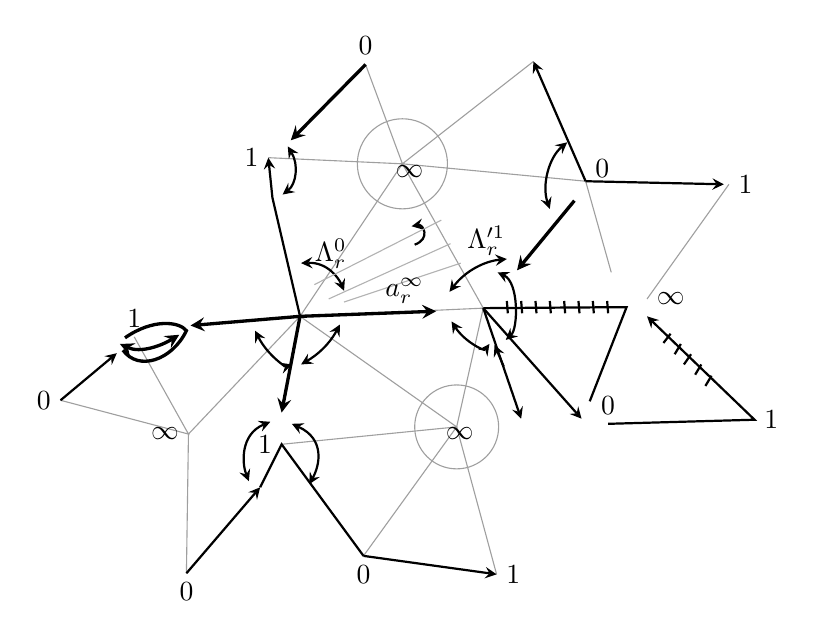
\begin{tikzpicture}[x=0.013cm,y=-0.013cm,>=stealth]
\draw[gray!75] (247,1588)--(378,1594)--(557,1611) (342,1497)--(378,1594)--(457,1735)--(278,1743)--(378,1594)--(506,1494);
\draw[gray!75] (116,1763)--(169,1858)--(44,1825) (169,1858)--(167,1994) (169,1858)--(278,1743)--(431,1851)--(260,1868);
\draw[gray!75] (457,1735)--(431,1851)--(340,1977) (431,1851)--(470,1995) (557,1611)--(582,1700) (617,1726)--(697,1614);
\draw[gray!75] (378,1594) circle (44);\draw[gray!75] (431,1851) circle (41);
\draw[very thick,->] (342,1497)--(269,1571);\draw[thick,->] (278,1743)--(251,1627)--(247,1588);
\draw[thick,<->] (266,1577)..controls(277,1595)and(274,1614)..(261,1624);
\draw[thick,->] (557,1611)--(506,1494);
\draw[thick,<->] (539,1573)..controls(521,1588)and(514,1615)..(522,1638);
\draw[thick,->] (557,1611)--(692,1614);
\draw[very thick,->] (546,1630)--(490,1698);
\draw[very thick,->] (278,1743)--(411,1738);
\draw[very thick,->] (278,1743)--(260,1837);
\draw[very thick,->] (278,1743)--(171,1752);
\draw[thick,<->] (279,1691)..controls(305,1690)and(316,1706)..(321,1718);
\draw[thick,<->] (424,1719)..controls(440,1698)and(459,1689)..(480,1687);
\draw[thick,<->] (234,1757)..controls(247,1782)and(264,1792)..(270,1790);
\draw[thick,<->] (279,1790)..controls(301,1777)and(310,1764)..(317,1751);
\draw[thick,->] (457,1735)--(494,1843);
\draw[thick,->] (457,1735)--(553,1843);
\draw[thick,->] (579,1848)--(722,1844)--(617,1743);
\draw[thick] (457,1735)--(597,1734)--(561,1826);
\foreach \x in {480,494,508,522,536,550,564,578}{\draw[thick] (\x,1728)--(\x+1,1740);}
\draw[thick] (640,1760)--(633,1769) (650,1770)--(644,1780) (660,1780)--(653,1790) (670,1790)--(664,1800) (680,1801)--(674,1811);
\draw[thick,<->] (471,1700)..controls(492,1710)and(491,1755)..(479,1766);
\draw[thick,<->] (426,1748)..controls(439,1768)and(458,1777)..(463,1770);
\draw[thick,->] (477,1792)--(468,1771);
\draw[thick,->] (167,1994)--(239,1910);\draw[thick] (239,1910)--(260,1868)--(340,1977);
\draw[thick,->] (340,1977)--(470,1995);
\draw[thick,<->] (249,1846)..controls(220,1858)and(221,1886)..(228,1904);
\draw[thick,<->] (270,1848)..controls(303,1863)and(297,1889)..(287,1907);
\draw[thick,->] (44,1825)--(99,1779);
\draw[very thick,<->] (102,1770)..controls(122,1779)and(142,1772)..(160,1761);
\draw[very thick] (107,1764)..controls(134,1745)and(160,1748)..(167,1757)..controls(153,1786)and(120,1797)..(105,1776);
\draw[thick,->] (390,1673)..controls(406,1667)and(398,1653)..(387,1655);
\draw[gray!60] (292,1712)--(416,1649) (306,1726)--(425,1672) (321,1729)--(435,1691);
\node[above] at (342,1497) {$0$};\node[left] at (247,1588) {$1$};\node at (385,1602) {$\infty$};
\node[right] at (557,1599) {$0$};\node[right] at (697,1614) {$\unsure{1}$};\node[right] at (617,1726) {$\infty$};
\node[above] at (579,1848) {$0$};\node[right] at (722,1844) {$1$};\node[right] at (470,1995) {$1$};
\node[below] at (340,1977) {$0$};\node[below] at (167,1994) {$0$};\node[left] at (260,1868) {$1$};
\node[left] at (169,1858) {$\infty$};\node[left] at (44,1825) {$0$};\node[above] at (116,1763) {$1$};\node at (434,1858) {$\infty$};
\node at (308,1682) {$\Lambda_r^0$};\node at (460,1669) {$\Lambda_r^{\prime1}$};\node at (380,1718) {$a_r^\infty$};
\end{tikzpicture}
}
\margin{pavage par des \inserted{faces} polygonales de centre des sommets de type $\infty$ --- les coins de ces polygones étant arrondis pour éviter les trous}

c'est donc directement exprimé comme un groupoïde libre. Cela fait trois autres présentations de $\Pi_1(X)$, mais sur des ens. de sommets différents, savoir $\Pi_1(\widetilde{X}^{\substack{*\\*}*},S-S_i)$, pour $i=\infty$ (cas explicité) ou $0$ ou $1$.

\mspage{119}
